\chapter{Конструкторская часть}

В этой части представляются требования к программе, алгоритм визуализации сцены, выбранные типы и структуры данных, диаграмма классов.

\section{Требования к программе}

Программа должна обладать графическим интерфейсом, который позволит пользователю:
\begin{itemize}[label=--]
	\item изменять геометрические и спектральные характеристики модели многогранника;
	\item изменять положение модели многогранника в пространстве;
	\item изменять положение камеры в пространстве;
\end{itemize}

Разработанная программа должна выполнять следующие требования:
\begin{itemize}[label=--]
	\item источник света должен создаваться при запуске;
	\item в пространстве может быть только один источник света;
	\item в пространстве может быть только одна камера;
	\item программа обязана правильно обрабатывать некорректные вводимые данные.
\end{itemize}

\section{Общий алгоритм визуализации сцены}

На рисунке~\ref{fig:scene-visualization} представлен алгоритм, который генерирует изображение. Он принимает на вход геометрические и спектральные параметры моделей, характеристики камеры, данные об источнике света и его спектральные свойства, а на выходе предоставляет визуализированную сцену на экране.

\begin{figure}[h] 
	\centering
	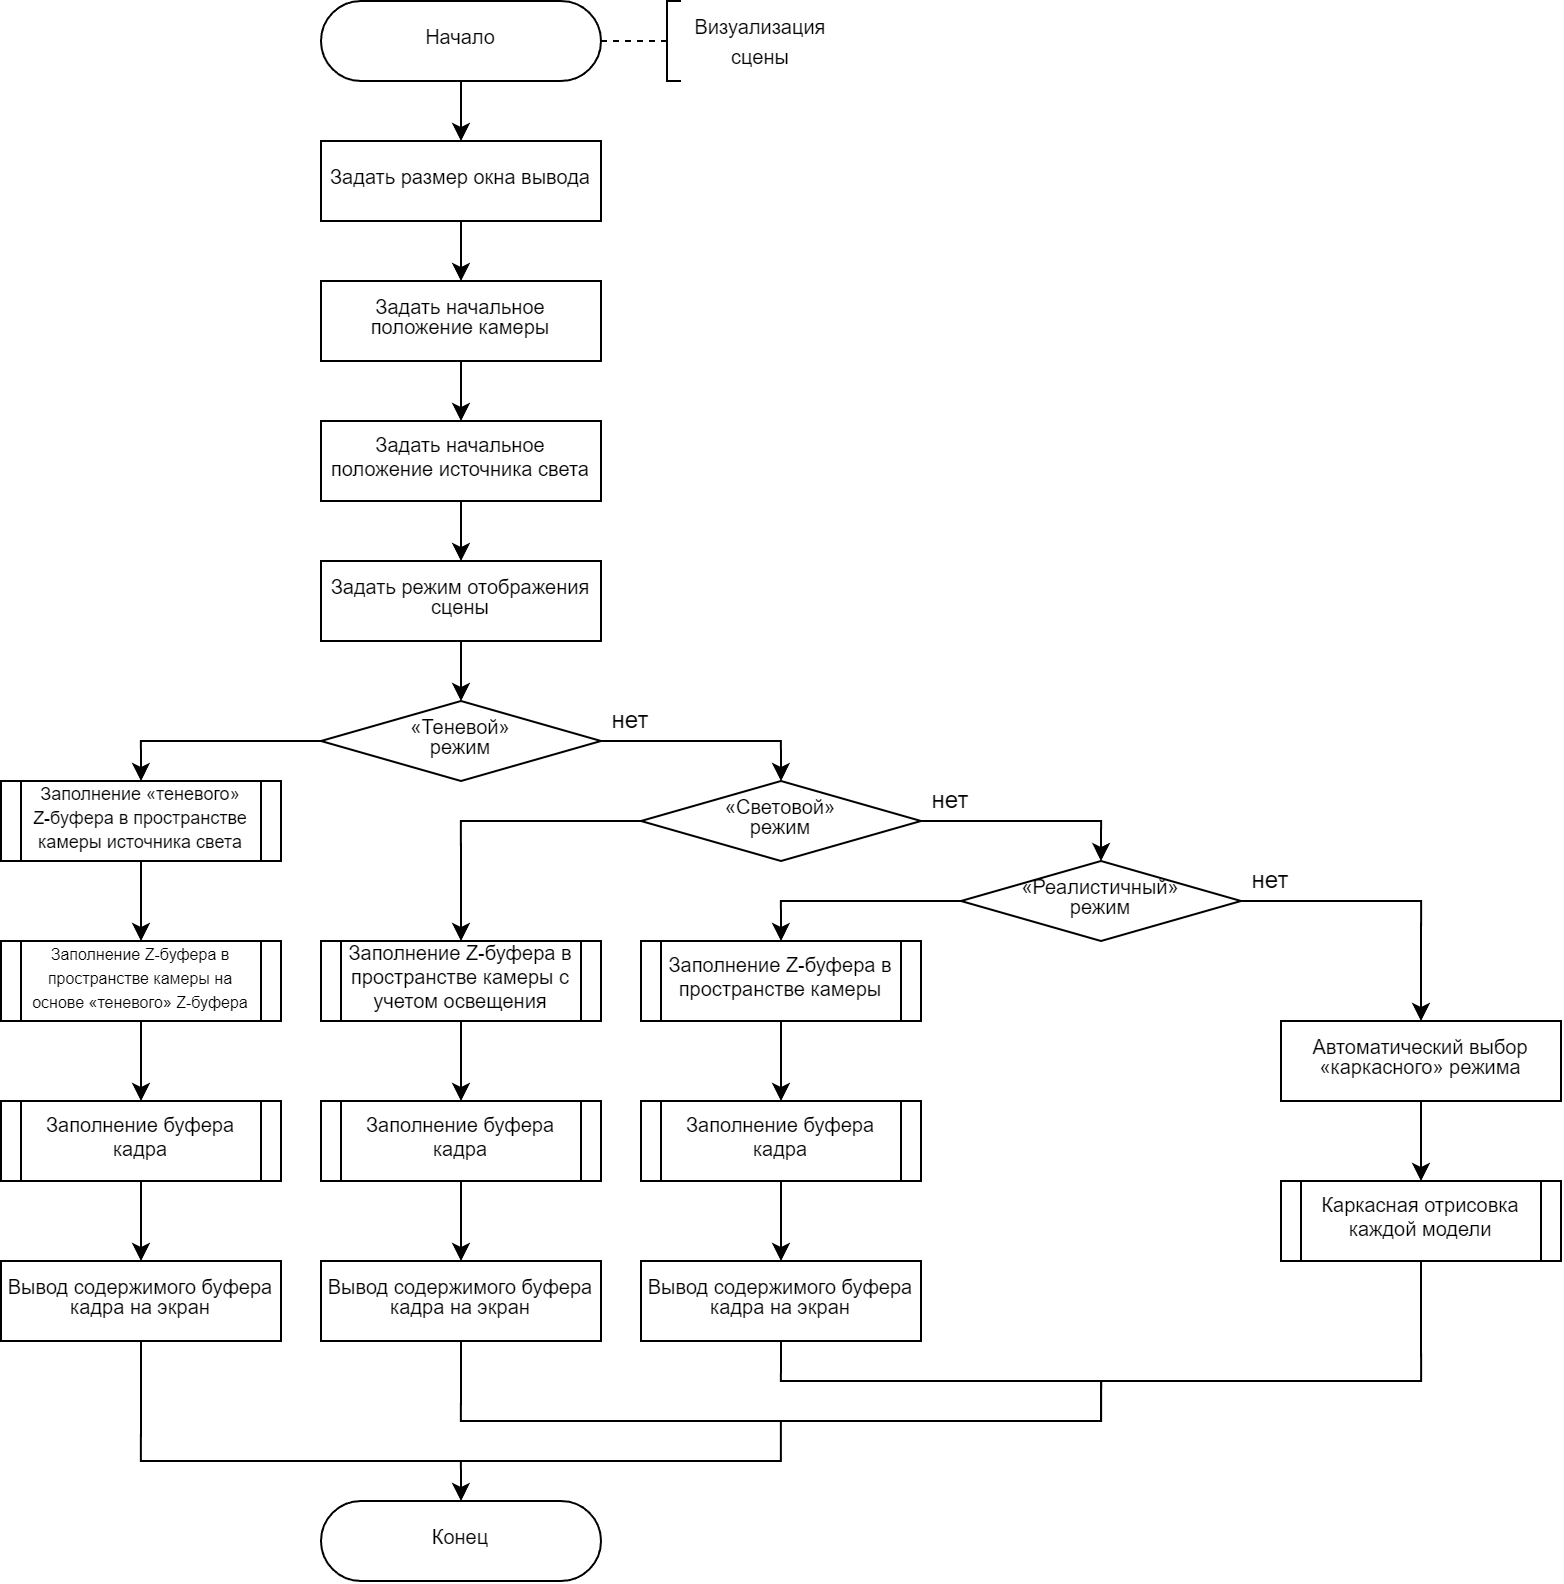
\includegraphics[width=0.9\textwidth]{images/scene-visualization.png}
	\caption{Общий алгоритм визуализации сцены} 
	\label{fig:scene-visualization} 
\end{figure}

Более подробный алгоритм визуализации сцены в <<теневом>> режиме отображения сцены при инициализированной сцене представлен на рисунке~
\ref{fig:shadow-mod}.
\begin{figure}[h] 
	\centering
	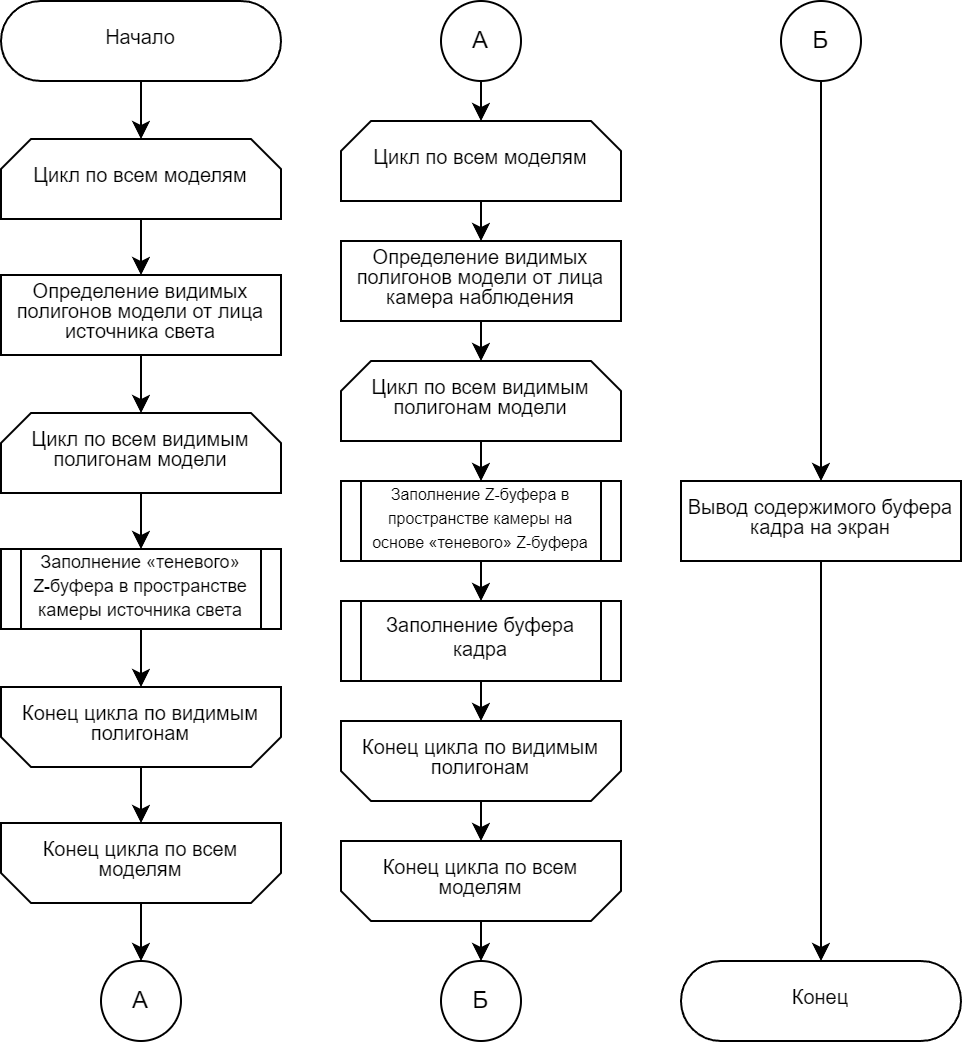
\includegraphics[width=1\textwidth]{images/shadow-mod.png}
	\caption{Общий алгоритм визуализации сцены в <<теневом>> режиме при инициализированной сцене} 
	\label{fig:shadow-mod} 
\end{figure}

Более подробный алгоритм визуализации сцены в <<световом>>, <<реалистичном>> и <<каркасном>> режимах отображения сцены при инициализированной сцене представлены на рисунке~\ref{fig:other-mods}.
\begin{figure}[h] 
	\centering
	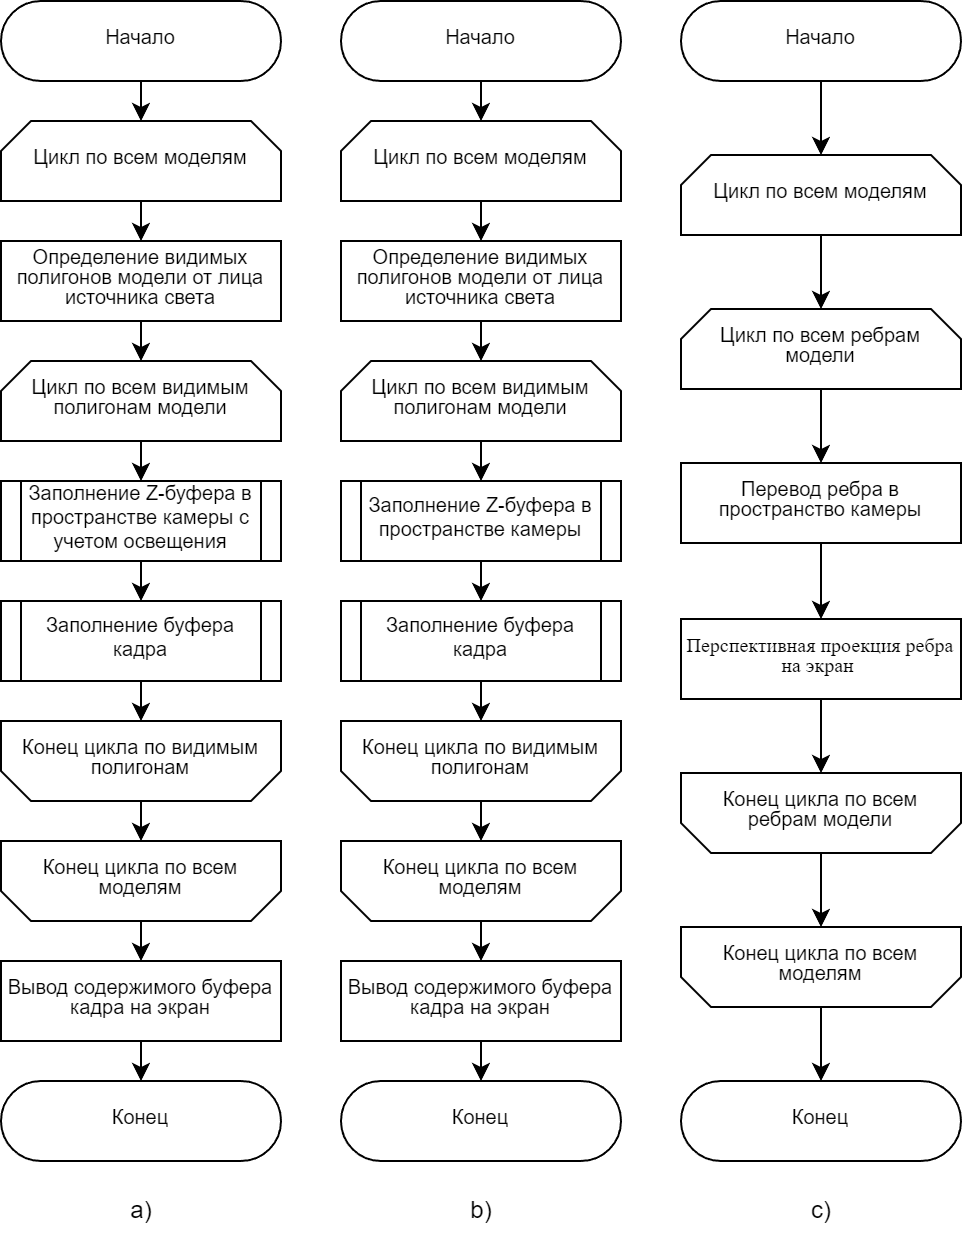
\includegraphics[width=1\textwidth]{images/other-mods.png}
	\caption{Общий алгоритм визуализации сцены в иных режимах при инициализированной сцене: <<световой>> (a), <<реалистичный>> (b), <<каркасный>> (c)} 
	\label{fig:other-mods} 
\end{figure}


\clearpage

\section{Афинные преобразования}

...

\section{Перспективная проекция}

...

\subsection{Пирамида видимости}

...

\subsection{Мировое пространство}

...

\subsection{Пространство камеры}

...

\subsection{Проекция на плоскость изображения}

...

\section{Невидимые грани}

...

\section{Схемы алгоритмов}

...

\section{Выбор типов и структур данных}

...

\section{Диаграмма классов}

...

\section{Вывод}

<что сделали в конструкторке и получили в результате, кратко>

\clearpage
